\begin{figure}
\centering

% Created by tikzDevice version 0.12.5 on 2023-11-28 18:56:48
% !TEX encoding = UTF-8 Unicode
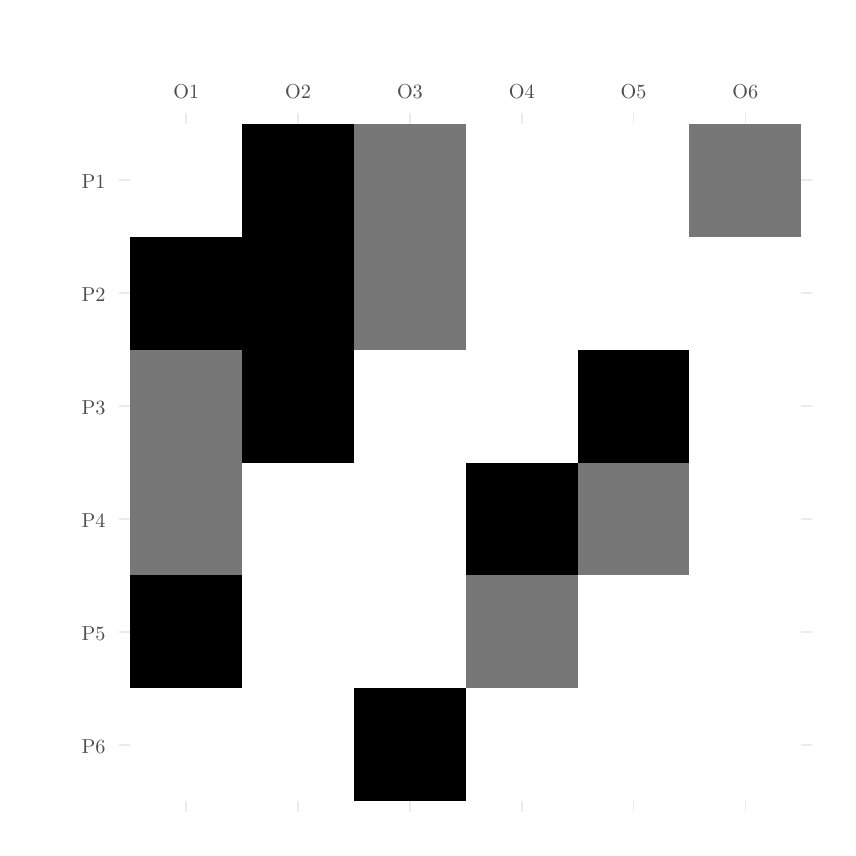
\begin{tikzpicture}[x=1pt,y=1pt]
\definecolor{fillColor}{RGB}{255,255,255}
\path[use as bounding box,fill=fillColor,fill opacity=0.00] (0,0) rectangle (289.08,289.08);
\begin{scope}
\path[clip] ( 33.08,  5.50) rectangle (283.58,258.39);
\definecolor{drawColor}{gray}{0.92}

\path[draw=drawColor,line width= 0.6pt,line join=round] ( 33.08, 29.97) --
	(283.58, 29.97);

\path[draw=drawColor,line width= 0.6pt,line join=round] ( 33.08, 70.76) --
	(283.58, 70.76);

\path[draw=drawColor,line width= 0.6pt,line join=round] ( 33.08,111.55) --
	(283.58,111.55);

\path[draw=drawColor,line width= 0.6pt,line join=round] ( 33.08,152.34) --
	(283.58,152.34);

\path[draw=drawColor,line width= 0.6pt,line join=round] ( 33.08,193.13) --
	(283.58,193.13);

\path[draw=drawColor,line width= 0.6pt,line join=round] ( 33.08,233.92) --
	(283.58,233.92);

\path[draw=drawColor,line width= 0.6pt,line join=round] ( 57.32,  5.50) --
	( 57.32,258.39);

\path[draw=drawColor,line width= 0.6pt,line join=round] ( 97.73,  5.50) --
	( 97.73,258.39);

\path[draw=drawColor,line width= 0.6pt,line join=round] (138.13,  5.50) --
	(138.13,258.39);

\path[draw=drawColor,line width= 0.6pt,line join=round] (178.53,  5.50) --
	(178.53,258.39);

\path[draw=drawColor,line width= 0.6pt,line join=round] (218.94,  5.50) --
	(218.94,258.39);

\path[draw=drawColor,line width= 0.6pt,line join=round] (259.34,  5.50) --
	(259.34,258.39);
\definecolor{fillColor}{RGB}{255,255,255}

\path[fill=fillColor] ( 37.12,213.53) rectangle ( 77.53,254.32);
\definecolor{fillColor}{RGB}{0,0,0}

\path[fill=fillColor] ( 77.53,213.53) rectangle (117.93,254.32);
\definecolor{fillColor}{RGB}{119,119,119}

\path[fill=fillColor] (117.93,213.53) rectangle (158.33,254.32);
\definecolor{fillColor}{RGB}{255,255,255}

\path[fill=fillColor] (158.33,213.53) rectangle (198.73,254.32);

\path[fill=fillColor] (198.73,213.53) rectangle (239.14,254.32);
\definecolor{fillColor}{RGB}{119,119,119}

\path[fill=fillColor] (239.14,213.53) rectangle (279.54,254.32);
\definecolor{fillColor}{RGB}{0,0,0}

\path[fill=fillColor] ( 37.12,172.74) rectangle ( 77.53,213.53);

\path[fill=fillColor] ( 77.53,172.74) rectangle (117.93,213.53);
\definecolor{fillColor}{RGB}{119,119,119}

\path[fill=fillColor] (117.93,172.74) rectangle (158.33,213.53);
\definecolor{fillColor}{RGB}{255,255,255}

\path[fill=fillColor] (158.33,172.74) rectangle (198.73,213.53);

\path[fill=fillColor] (198.73,172.74) rectangle (239.14,213.53);

\path[fill=fillColor] (239.14,172.74) rectangle (279.54,213.53);
\definecolor{fillColor}{RGB}{119,119,119}

\path[fill=fillColor] ( 37.12,131.95) rectangle ( 77.53,172.74);
\definecolor{fillColor}{RGB}{0,0,0}

\path[fill=fillColor] ( 77.53,131.95) rectangle (117.93,172.74);
\definecolor{fillColor}{RGB}{255,255,255}

\path[fill=fillColor] (117.93,131.95) rectangle (158.33,172.74);

\path[fill=fillColor] (158.33,131.95) rectangle (198.73,172.74);
\definecolor{fillColor}{RGB}{0,0,0}

\path[fill=fillColor] (198.73,131.95) rectangle (239.14,172.74);
\definecolor{fillColor}{RGB}{255,255,255}

\path[fill=fillColor] (239.14,131.95) rectangle (279.54,172.74);
\definecolor{fillColor}{RGB}{119,119,119}

\path[fill=fillColor] ( 37.12, 91.16) rectangle ( 77.53,131.95);
\definecolor{fillColor}{RGB}{255,255,255}

\path[fill=fillColor] ( 77.53, 91.16) rectangle (117.93,131.95);

\path[fill=fillColor] (117.93, 91.16) rectangle (158.33,131.95);
\definecolor{fillColor}{RGB}{0,0,0}

\path[fill=fillColor] (158.33, 91.16) rectangle (198.73,131.95);
\definecolor{fillColor}{RGB}{119,119,119}

\path[fill=fillColor] (198.73, 91.16) rectangle (239.14,131.95);
\definecolor{fillColor}{RGB}{255,255,255}

\path[fill=fillColor] (239.14, 91.16) rectangle (279.54,131.95);
\definecolor{fillColor}{RGB}{0,0,0}

\path[fill=fillColor] ( 37.12, 50.37) rectangle ( 77.53, 91.16);
\definecolor{fillColor}{RGB}{255,255,255}

\path[fill=fillColor] ( 77.53, 50.37) rectangle (117.93, 91.16);

\path[fill=fillColor] (117.93, 50.37) rectangle (158.33, 91.16);
\definecolor{fillColor}{RGB}{119,119,119}

\path[fill=fillColor] (158.33, 50.37) rectangle (198.73, 91.16);
\definecolor{fillColor}{RGB}{255,255,255}

\path[fill=fillColor] (198.73, 50.37) rectangle (239.14, 91.16);

\path[fill=fillColor] (239.14, 50.37) rectangle (279.54, 91.16);

\path[fill=fillColor] ( 37.12,  9.58) rectangle ( 77.53, 50.37);

\path[fill=fillColor] ( 77.53,  9.58) rectangle (117.93, 50.37);
\definecolor{fillColor}{RGB}{0,0,0}

\path[fill=fillColor] (117.93,  9.58) rectangle (158.33, 50.37);
\definecolor{fillColor}{RGB}{255,255,255}

\path[fill=fillColor] (158.33,  9.58) rectangle (198.73, 50.37);

\path[fill=fillColor] (198.73,  9.58) rectangle (239.14, 50.37);

\path[fill=fillColor] (239.14,  9.58) rectangle (279.54, 50.37);
\end{scope}
\begin{scope}
\path[clip] (  0.00,  0.00) rectangle (289.08,289.08);
\definecolor{drawColor}{gray}{0.30}

\node[text=drawColor,anchor=base,inner sep=0pt, outer sep=0pt, scale=  0.73] at ( 57.32,263.34) {O1};

\node[text=drawColor,anchor=base,inner sep=0pt, outer sep=0pt, scale=  0.73] at ( 97.73,263.34) {O2};

\node[text=drawColor,anchor=base,inner sep=0pt, outer sep=0pt, scale=  0.73] at (138.13,263.34) {O3};

\node[text=drawColor,anchor=base,inner sep=0pt, outer sep=0pt, scale=  0.73] at (178.53,263.34) {O4};

\node[text=drawColor,anchor=base,inner sep=0pt, outer sep=0pt, scale=  0.73] at (218.94,263.34) {O5};

\node[text=drawColor,anchor=base,inner sep=0pt, outer sep=0pt, scale=  0.73] at (259.34,263.34) {O6};
\end{scope}
\begin{scope}
\path[clip] (  0.00,  0.00) rectangle (289.08,289.08);
\definecolor{drawColor}{gray}{0.30}

\node[text=drawColor,anchor=base east,inner sep=0pt, outer sep=0pt, scale=  0.73] at ( 28.13, 26.94) {P6};

\node[text=drawColor,anchor=base east,inner sep=0pt, outer sep=0pt, scale=  0.73] at ( 28.13, 67.73) {P5};

\node[text=drawColor,anchor=base east,inner sep=0pt, outer sep=0pt, scale=  0.73] at ( 28.13,108.52) {P4};

\node[text=drawColor,anchor=base east,inner sep=0pt, outer sep=0pt, scale=  0.73] at ( 28.13,149.31) {P3};

\node[text=drawColor,anchor=base east,inner sep=0pt, outer sep=0pt, scale=  0.73] at ( 28.13,190.10) {P2};

\node[text=drawColor,anchor=base east,inner sep=0pt, outer sep=0pt, scale=  0.73] at ( 28.13,230.89) {P1};
\end{scope}
\end{tikzpicture}

\caption{\label{fig:test}Test}

\end{figure}